\documentclass{article}
\usepackage{styles/project_style} % Assuming you have this style file
\addbibresource{references/projects.bib}

\title{Cellular Automata Simulation of Granular Flow}

\begin{document}
\maketitle

\section{Introduction}

A \emph{cellular automaton} (CA) is a grid of cells, each of which holds one of a finite set of states. Time advances in discrete steps, and at each step every cell updates its state simultaneously according to a rule that depends only on its own state and the states of its nearby neighbors (for example, the four orthogonal neighbors in a square grid). Although each rule is simple and local, when repeated over many steps these updates can produce complex, large‑scale patterns.

\begin{figure}[htbp]
  \centering
  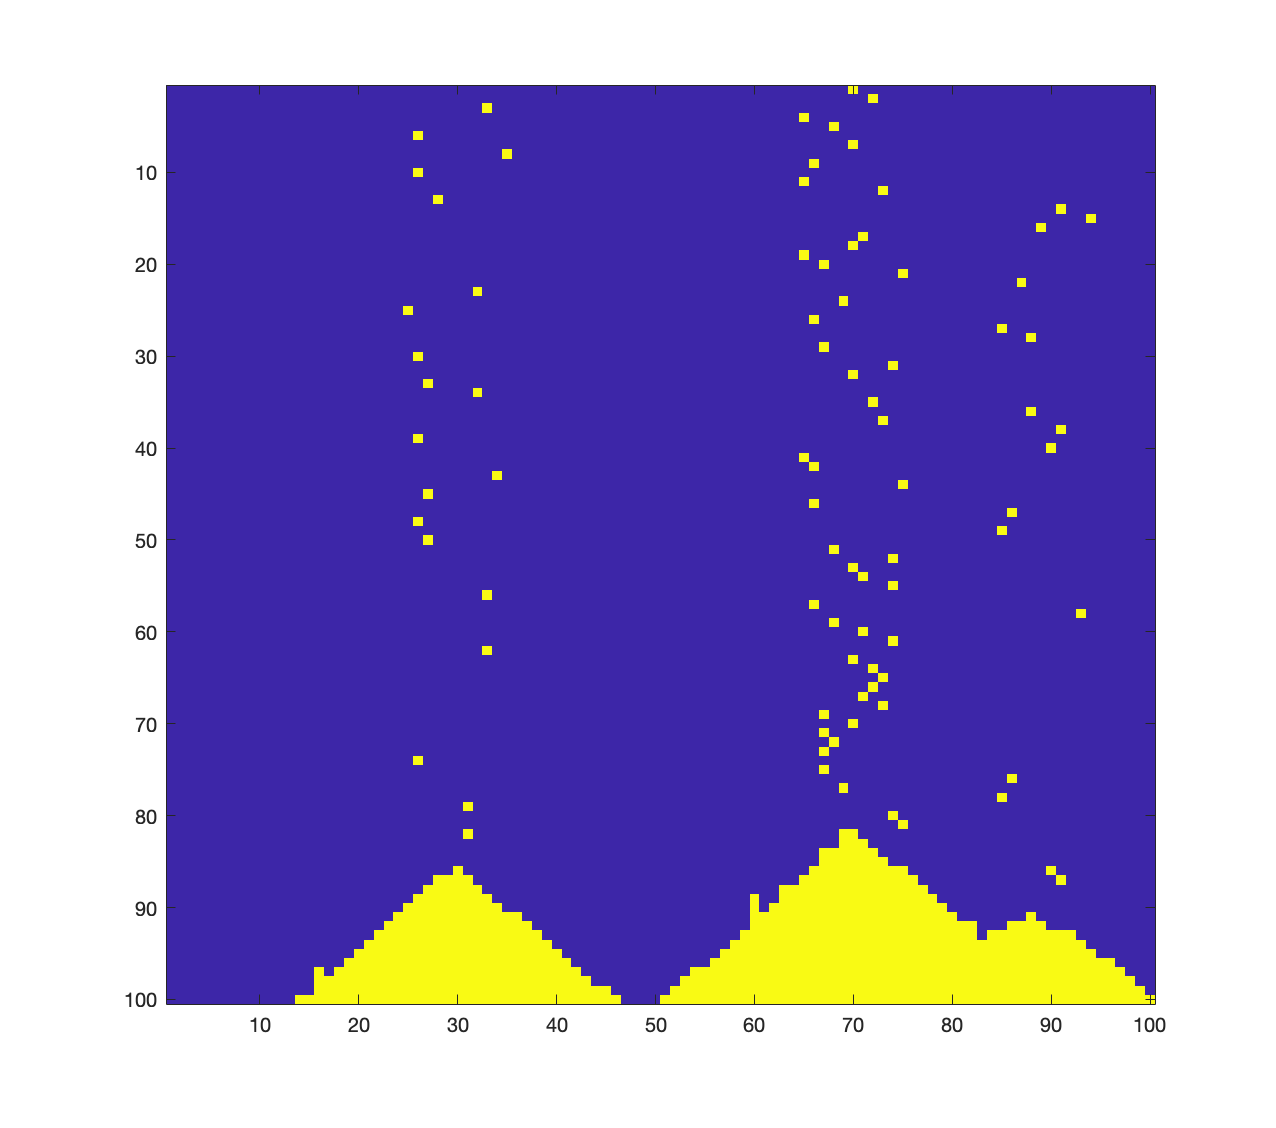
\includegraphics[width=0.4\textwidth]{projects/granular_flow/images/sand.png}
  \caption{Illustration of simple implementation of granular flow using celluar automata implemented in Matlab}
  \label{fig:allee-effects}
\end{figure}


Key characteristics of cellular automata are:
\begin{itemize}
  \item \textbf{Discrete space and time:} The grid has a fixed shape (e.g.\ square, hexagon) and cells update in lockstep at each time step.
  \item \textbf{Finite states:} Each cell can take one of a limited number of values (often just two, such as 0 or 1).
  \item \textbf{Local rules:} A cell’s next state is determined by a fixed rule applied to its neighborhood.
  \item \textbf{Parallel update:} All cells compute their next state at the same time, avoiding bias from sequential updates.
\end{itemize}

Early work by John von Neumann explored how CAs could model self‑replication, and Stephen Wolfram classified one‑dimensional “elementary” automata (256 possible rules) into four behavior classes, from uniform to chaotic to complex. In two dimensions, Conway’s Game of Life uses binary states and an eight‑cell neighborhood to generate stable patterns (“still lifes”), oscillators, and moving structures (“gliders”), even proving to be capable of universal computation.

Cellular automata are applied in many fields because they can mimic collective dynamics without solving complicated equations:
\begin{itemize}
  \item \textbf{Physics:} Lattice gas models simulate fluid and gas flow.
  \item \textbf{Biology:} Pattern formation in seashells or the spread of electrical activity in neural tissue.
  \item \textbf{Epidemiology:} Disease transmission models on networks of individuals.
  \item \textbf{Social sciences:} Models of urban growth, civil unrest, or opinion dynamics.
  \item \textbf{Cryptography:} Pseudorandom number generators and error‑correcting codes based on CA rules.
\end{itemize}

In the following sections, we will employ a two‑dimensional CA to simulate granular materials—such as sand and water—under gravity. By specifying simple rules for how particles fall, slide, and settle, we can reproduce behaviors like dune formation, channel carving, and multi‑phase flow, all within a purely discrete framework.


\section{Granular Automaton vs.\ Real‑World Granular Flow}

In physics, granular flow is often modeled via discrete element methods (DEM) or continuum approaches, which resolve interparticle forces and contact dynamics. Our cellular automaton is an abstraction: each grid cell holds at most one particle, and simple neighbor‑based rules drive movement and interaction. While less detailed than DEM, this approach highlights emergent behavior from minimal rules and is computationally efficient for large grids.

In computer game, for example indie title \textit{Noita}—a similar CA framework is used to simulate thousands of interacting particles in real time. Each pixel in the game world represents a cell that can contain materials like sand, water, oil or lava. Simple update rules (falling, sliding, mixing, phase changes) are applied in parallel each frame, producing complex effects such as fluid mixing, erosion of terrain, and chain reactions (e.g.\ oil igniting lava). This pixel‑based CA enables dynamic, unpredictable gameplay without heavy physics engines, allowing artists and designers to craft emergent scenarios that feel both natural and novel.

\section{Core Particle Behavior}

At each discrete time step, every particle on the grid evaluates its local neighborhood and updates according to the following sequence of rules.  Updates are computed into a separate array (\texttt{next\_grid}) so that all movements appear simultaneous and no particle is moved twice in a single step.

\begin{enumerate}
  \item \textbf{Gravity:}  
    \begin{itemize}
      \item If the cell directly below \((i+1, j)\) is empty, the particle moves there.
      \item This implements the basic downward pull of gravity.
    \end{itemize}
  \item \textbf{Diagonal Slide:}  
    \begin{itemize}
      \item If downward movement is blocked (cell below occupied), but either lower‑left \((i+1, j-1)\) or lower‑right \((i+1, j+1)\) is empty, the particle chooses one of these diagonals at random (or by predefined priority) and moves there.
      \item This allows particles to form sloped piles rather than rigid vertical columns.
    \end{itemize}
  \item \textbf{Lateral Shuffle (optional for fluids):}  
    \begin{itemize}
      \item For fluid‑like materials (water, oil), if neither downward nor diagonal moves are possible, check immediate horizontal neighbors \((i, j-1)\) and \((i, j+1)\).  
      \item If one side is empty (or lower than current cell), move there to simulate pooling and spreading.
    \end{itemize}
  \item \textbf{Settling:}  
    \begin{itemize}
      \item If no moves are available, the particle remains in place and is considered “settled” for this step.
      \item Settled particles contribute to local stability and can act as support for particles above.
    \end{itemize}
  \item \textbf{Material Interactions:}  
    \begin{itemize}
      \item After a move decision, apply any material‑specific reactions (e.g.\ water turning to vapor when in contact with lava, or sand eroding soft terrain beneath).
      \item Update both \texttt{next\_grid} and any auxiliary fields (temperature, erosion counters) accordingly.
    \end{itemize}
\end{enumerate}



\section{Algorithmic Representation}

\begin{enumerate}
  \item \textbf{Initialization:}  
    \begin{itemize}
      \item Allocate two 2D arrays, \texttt{grid} and \texttt{next\_grid}, of size \(H\times W\).
      \item Fill \texttt{grid} with initial particle types or empty cells according to scenario.
      \item Initialize auxiliary arrays for material properties (e.g.\ viscosity, temperature).
    \end{itemize}
  \item \textbf{Main Time Loop:}  Repeat for each time step \(t = 1, 2, \dots\)
    \begin{itemize}
      \item Copy or clear \texttt{next\_grid} to prepare for new states.
      \item \textbf{For each cell \((i,j)\) in \texttt{grid}:}
        \begin{enumerate}
          \item If \texttt{grid[i,j]} is empty, continue to next cell.
          \item Otherwise, compute possible moves in the order: gravity, diagonal slide, lateral shuffle.
          \item Execute the first valid move by writing the particle type into \texttt{next\_grid} at the destination and marking \((i,j)\) as empty in \texttt{next\_grid}.
          \item Apply any material‑specific updates (e.g.\ increment erosion counters, exchange heat).
        \end{enumerate}
      \item \textbf{Swap grids:}  
        \[
          \texttt{grid} \;\longleftarrow\; \texttt{next\_grid}.
        \]

    \end{itemize}
  \item \textbf{Termination:}  
    \begin{itemize}
      \item Stop after a fixed number of steps, percentage of fill, or when the system reaches a steady state (no particle has moved for \(k\) consecutive steps).
    \end{itemize}
\end{enumerate}


\section{Implementation Example}
The following code implements a simple agent-based sand simulation in MATLAB. The model represents a vertical 2D grid, where grains of sand fall from the top and follow gravity-based movement rules. This bottom-up approach allows grains to accumulate and form structures based on stochastic deposition and deterministic falling behavior.

The simulation proceeds in discrete time steps and involves three main components: parameter setup and grid initialization, the simulation loop, and two core functions that handle grain motion and generation.

Key parameters define the size of the grid and the stopping condition:

\begin{lstlisting}[caption={Parameters and Initialization}]
% ----- Parameters -----
grid_size = 100;
grain_count = 0;

% ----- Initialize grid -----
grid = zeros(grid_size);

% ----- Visualization setup -----
figure(1);
axis off;
drawnow;
\end{lstlisting}

The grid is initialized as a square matrix of zeros representing empty positions. Grains are represented by ones and visualized using \texttt{imagesc}. The simulation proceeds until 25\% of the grid is filled with sand grains. Each iteration updates the grid by moving grains based on gravity rules and introducing new grains at the top.

\begin{lstlisting}[caption={Simulation loop}]
while grain_count < round(grid_size^2/4)
    new_grid = grid;

    for row = grid_size-1:-1:1
        for col = 2:grid_size-1
            if grid(row, col) == 1
                new_grid = update_grain_position(grid, new_grid, row, col);
            end
        end
    end

    grid = new_grid;
    grid = generate_new_grain(grid, grid_size);
    grain_count = sum(grid(:));

    imagesc(grid);
    drawnow;
end
\end{lstlisting}

At each time step, the grains are updated from bottom to top to prevent overwriting falling grains. Each grain can fall straight down, down-left, or down-right depending on the availability of neighboring cells. After all grains are updated, a new grain is introduced near the center of the grid, simulating a falling stream.

The movement logic is implemented in the following function:
\newpage
\begin{lstlisting}[caption={Grain movement function}]
function new_grid = update_grain_position(grid, new_grid, row, col)
    if grid(row+1, col) == 0
        new_grid(row, col) = 0;
        new_grid(row+1, col) = 1;
    elseif grid(row+1, col-1) == 0
        new_grid(row, col) = 0;
        new_grid(row+1, col-1) = 1;
    elseif grid(row+1, col+1) == 0
        new_grid(row, col) = 0;
        new_grid(row+1, col+1) = 1;
    end
end
\end{lstlisting}

This function checks for available directions a grain can fall and updates the grid accordingly. Grains always prefer to fall straight down if possible, with diagonal directions as secondary options.

Grains are introduced at each time step using a randomized stream position. Note that this function is a bit complicated then necessary for a simple demonstration. The main goal is to have more naturally looking shapes. Having grain generation in a separate function allows for easy customation of the functuon. 

\begin{lstlisting}[caption={Grain generation function}]
function grid = generate_new_grain(grid, grid_size)
    plot_center = round(grid_size / 2);
    random_variation = randi([-5, 5]);

    stream_distance = round(grid_size / 5);
    stream_position_start = [2, 1, 1, 1, -1, -1];
    idx = randi(numel(stream_position_start));
    stream = stream_distance * stream_position_start(idx);

    grain_start = plot_center + stream + random_variation;
    grain_start = max(1, min(grid_size, grain_start));
    grid(1, grain_start) = 1;
end
\end{lstlisting}

This function introduces stochasticity into the model by varying both the stream direction and exact column position, simulating natural irregularity in sand deposition. The simulation captures how local movement rules and accumulation dynamics result in emergent macroscopic structures, a common feature in self-organizing systems such as granular flows and cellular automata.

\section{Literature}
\subsection{General introduction}
The topic is well discussed in several online resources. A blog mentioned is a good starting point. In addition several videos on YouTube on the topic. See:
\begin{itemize}
    \item \textcite{GranularFlow_Macuyiko2017part1}
    \item \textcite{GranularFlow_Macuyiko2017part2}
    \item \textcite{GranularFlow_Macuyiko2018part3}
    \item \textcite{GranularFlow_Macuyiko2020part4}
    \item \textcite{GranularFlow_Wheel2009}
    \item \textcite{GranularFlow_Pierre2020}
        
\end{itemize}

\subsection{Journal Club}
Here are several papers that can be discussed in the Journal Club presentation.
\begin{itemize}
    \item \textcite{GranularFlow_Baxter1990}
    \item \textcite{GranularFlow_Castro2021}
    \item \textcite{GranularFlow_Kozicki2005}
\end{itemize}

\printbibliography % Command to print the bibliography defined in references/projects.bib

\end{document}

